\chapter{Fornax实现细节分析}
\label{chap:detail}

本章从细节实现的角度出发,自顶而下地介绍了Fornax每个模块的具体实现。在第\ref{chap:impl}章中提到,API模块是Fornax与客户端交互的入口。因此对实现的具体细节分析,将从最顶层的API模块入手。

\section{Fornax初始化}

Fornax在实现上依赖很多外部的服务,其中包括MongoDB,Kafka,和Docker等。因此,如果要运行Fornax,必须有这些依赖的支持。为了实现依赖的可配置,Fornax采取了环境变量的方式定义这些依赖。表\ref{tab:env}列出了Fornax中所有的环境变量。其中前两项为MongoDB和Kafka服务所在的地址,通常是以IP或者域名的形式给出,而端口则是在两个服务启动时所在的默认端口。而DOCKER\_HOST和DOCKER\_HOST\_DIR是为了支持多个Docker Host做构建而定义的环境变量。而以REGISTRY为前缀的三个环境变量是与Docker Registry相关的配置,它们定义了地址与用户名密码,它们的作用会在之后进行更为详细的阐述。上面提到的环境变量是Fornax中为了解决依赖可配置而引入的,而其他的环境变量则是出于便于开发的目的,在此不做过多介绍。

在读取环境变量后,Fornax会将API模块中的所有API注册到一个HTTP服务器上,然后在主线程里运行该服务器,监听相应端口(默认为7099)。同时,Fornax会将额外启动一个线程来运行异步事件处理器的事件循环,事件循环可以被视为一个不会停止的循环,它接受一个通道(channel)的消息,并进行处理。还有一个WebSocket的服务器,同样会运行在一个独立的线程中,该线程主要负责将日志实时地推送给接收方。因此,在初始化后,Fornax会有三个线程在运行。

\begin{table}[!hpb]
  \centering
  \caption{Fornax环境变量配置}
  \label{tab:env}
  \begin{tabular}{ll} \toprule
    环境变量 & 描述 \\ \midrule
    MONGO\_DB\_IP & MongoDB服务地址 \\
    KAFKA\_SERVER\_IP & Kafka服务地址  \\
    DOCKER\_HOST & Docker Host地址  \\
    DOCKER\_HOST\_DIR & Docker Host目录 \\
    REGISTRY\_LOCATION & Docker Registry地址  \\
    REGISTRY\_USERNAME & Docker Registry用户名  \\
    REGISTRY\_PASSWORD & Docker Registry密码  \\
    DOCKER\_CERT\_PATH & Docker认证目录  \\
    ENABLE\_CAICLOUD\_AUTH & 是否开启用户认证  \\ \bottomrule
  \end{tabular}
\end{table}

\section{API模块实现}

% 有error?
\begin{table}[!hpb]
  \centering
  \caption[tab:api]{Fornax REST API}
  \begin{tabular}{lll} \toprule
    URL & 方法 & 描述 \\ \midrule
    /\{user\_id\}/services & POST & 创建新的服务 \\
    /\{user\_id\}/services & GET & 获得所有服务 \\
    /\{user\_id\}/services/\{service\_id\} & GET & 根据ServiceID查询服务 \\
    /\{user\_id\}/services/\{service\_id\} & DELETE & 根据ServiceID删除服务 \\
    /\{user\_id\}/services/\{code\_repository\}/requesttoken & GET & 根据用户请求私有仓库的Token \\
    /services/\{code\_repository\}/authcallback & GET & 授权的回调处理 \\
    /\{user\_id\}/services/\{code\_repository\}/listrepo & GET & 使用请求的Token列出所有仓库 \\
    /\{user\_id\}/services/\{code\_repository\}/logout & GET & 从Fornax中登出该Token \\
    /\{user\_id\}/versions & POST & 创建新的版本 \\
    /\{user\_id\}/versions/\{version\_id\} & GET & 根据ServiceID查询版本 \\
    /\{user\_id\}/versions/\{version\_id\}/logs & GET & 获得日志(默认无WebSocket支持)\\
    /\{user\_id\}/services/\{service\_id\}/versions & GET & 列出一个服务对应的所有版本 \\
    /apidocs & GET & API文档(默认不生成) \\ \bottomrule
  \end{tabular}
\end{table}

Fornax中的服务,是以REST API的形式暴露给外界的,而API模块就是对于REST API的封装。在之前的章节中提到,服务和版本是Fornax中两个最重要的实体概念。因此在REST API中这两个模型也是最主要的数据实体。Fornax所有的API在表\ref{tab:api}中列出。

% \begin{figure}[!htp]
%   \centering
%   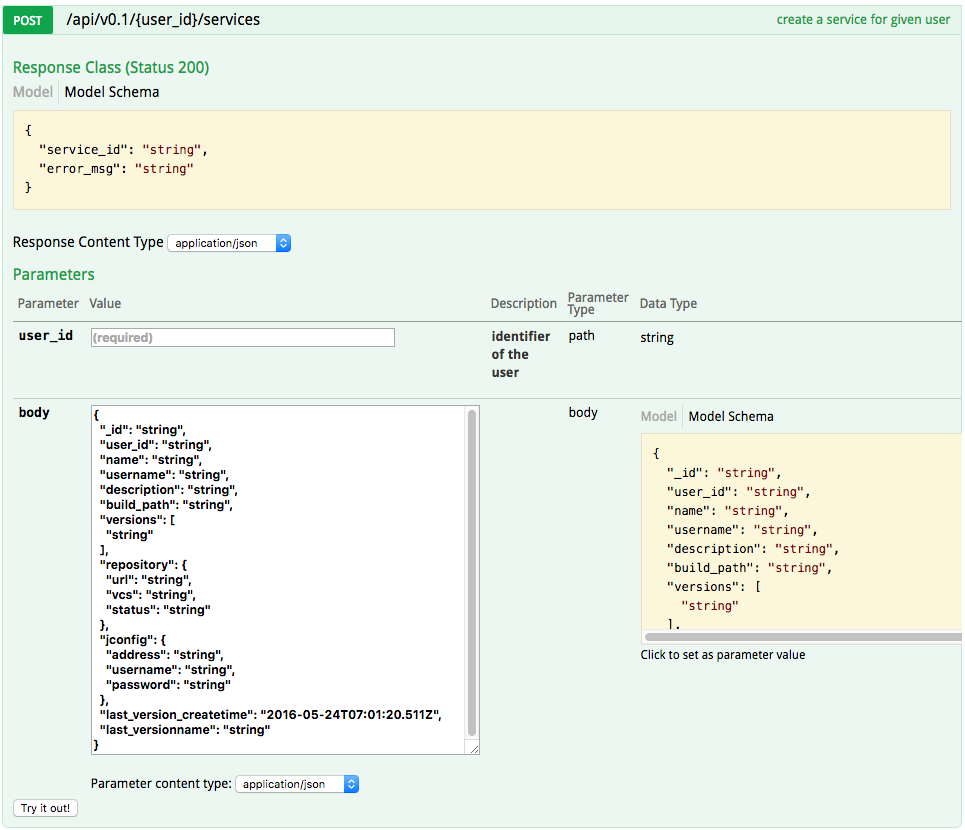
\includegraphics[width=0.9\textwidth]{detail/apidoc.png}
%   \bicaption[fig:api]{Fornax API文档图}{Fornax API文档图}{Fig}{}
% \end{figure}

通过定义了REST API,并将其与相应的逻辑处理器关联起来,最终以HTTP服务器的方式运行起来,以实现对外服务的功能。值得一提的是,Fornax在API模块中也实现了一项对开发者而言比较友好功能,即根据代码来直接生成REST API文档,而不再像是传统的方式那样,手动地维护一份API文档以供参考。在代码中定义REST API的部分,通过加入少量的说明,Fornax可以在运行时通过Flag的方式来决定是否将在运行的同时在/apidocs下生成一份API文档。首先,根据Fornax中原本的代码,会首先生成一个JSON格式的API规约,然后利用著名的API工具Swagger,产生一份人类可阅读的,HTML格式的文档。在API文档中不仅包括API的请求参数,以及返回的参数,还可以浏览到在代码中对应的相应的模型的定义,同时也可以直接通过文档发送请求,测试API的可用性。API模块的这一功能,使得外部与Fornax交互时可以感知到最新的接口,不会出现因为长时间没有维护API文档而导致的一系列问题。

\section{异步事件管理模块}

异步事件管理模块,是处理服务与版本创建的模块。在Fornax最初的设计中,所有的逻辑处理都是在主线程中完成,后来随着服务与版本在创建时的复杂性的提高,这样的设计不能满足需求,因此引入了异步事件管理模块,将创建服务与版本的过程异步化,使得它们不会阻塞主进程。

异步事件管理模块的运行模型是传统的事件循环模型,异步事件管理模块的运行过程可以抽象为一个永远不会退出的循环,当收到来自API模块发送到来的消息时,会调用相关的处理器来处理该事件,并且会在处理结束后执行定义的钩子函数,来进行数据库操作,或者收尾工作等等。采取事件循环的模型,使得Fornax在请求量巨大时,不会因为同时处理多个构建任务而崩溃。而这样的模型使得Fornax支持通过拒绝一部分请求,或者限制最大请求队列长度等方式来解决请求过载的问题。

% \begin{lstlisting}[caption={抽象后的异步事件管理器结构与实现}]
% type AsyncManager struct {
% 	operations map[Operation]OperationHandler
% 	events map[EventID]*Event
% 	newEvents chan *Event
% 	deleteEvents chan *Event
% 	lock sync.Mutex
% }

% func (am *AsyncManager) Start() {
% 	go func() {
% 		for {
% 			select {
% 			case event := <-am.newEvents:
% 				go func() {
% 					operationHandler, ok := am.operations[event.Operation]
% 					err := operationHandler(event)
% 					event.Lock.Lock()
% 					defer event.Lock.Unlock()
% 					// Deal with the error and call the post hook function.
% 				}()
% 			case event := <-am.deleteEvents:
% 				delete(am.events, event.EventID)
% 			}
% 		}
% 	}()
% }
% \end{lstlisting}

\begin{algorithm}
\caption{异步事件管理模块事件循环}
\label{algo:eventloop}
\begin{algorithmic}
\LOOP
\IF {there is a new event sent to the async event manager} 
\STATE Create a new goroutine and call the handler function for the event.
\ELSIF {There is a command to delete a event}
\STATE Delete the event from the manager.
\ENDIF 
\ENDLOOP
\end{algorithmic}
\end{algorithm}

在其他语言中实现这样事件驱动的模型,是比较复杂的。而在go语言中,因为其对于通道(channel)和轻量级线程(goroutine)的支持,所以实现这样一个模型非常简单,这也是Fornax最终采取这样的模型进行异步化创建服务和版本任务的原因之一。异步事件管理器的数据结构如代码所示,其由一个以操作为键,以处理器函数为值的图、一个以事件的唯一标识符为键,以对应的事件的指针为值的图、以及两个通道和一个互斥锁构成。在执行Start函数时,首先会创建一个新的线程,并在该线程中进入一个无限循环,在循环中,会使用go语言中的select特性,来进行对事件的监听。如果接收到新的事件,就会去operations中寻找对应的处理器函数,并调用其进行处理。目前只有两种有意义的操作类型,即创建服务和创建版本,而因为两者之间不存在数据竞争,因此在进行处理时不需要加锁,只有在涉及到对事件本身的属性的修改时才需要加锁。

异步事件管理模块与Docker管理模块、持续集成管理模块、和版本控制系统管理模块在处理器函数中进行交互。在创建服务的过程中,Fornax会将用户指定的仓库Clone到本地,进行简单地校验,然后在结束时会将服务的元数据写入数据库。因此在创建服务的处理器函数中,会与版本控制系统管理模块进行交互。而在创建版本时,则会与三个模块都有交互。

\section{Docker管理模块}

Docker管理模块是在执行镜像的构建与打包时会被调用的模块。Docker管理模块会负责与Docker Host交互,当有创建版本的请求被发起时,会涉及到对于版本镜像的构建和发布。因此,Docker管理模块需要维护在构建与发布镜像时的所有信息。而且在构建镜像时,也需要对Docker Registry进行设定,保证用户可以从其可见的基础镜像中构建新的镜像。

% \begin{lstlisting}[caption={Docker管理模块结构}]
% type DockerManager struct {
%   client     *docker_client.Client
%   registry   string
%   authConfig *AuthConfig
%   endPoint   string
% }
% \end{lstlisting}

Docker管理模块的结构相对于其他模块而言比较简单,其中最主要的对象是Docker Client的抽象对象,该对象会负责与Docker Host进行交互,而诸如构建、发布等功能也是通过该对象进行的。而其他的对象,是在执行构建与发布时需要用到的参数。在构建与发布时,用户通常会将镜像推送到自建的Docker Registry上,这样的需求要求在进行构建与发布时,允许用户来指定一些用来认证的配置,以保证推送的成功。

\section{版本管理系统管理模块}

版本管理系统管理模块是唯一一个在创建服务与创建版本时都会使用的模块。不同于其他类型的模块,它们只有一种实现,版本管理系统管理模块因为需要适配多种版本管理系统,因此有着更高的抽象。

\begin{figure}[!htp]
  \centering
  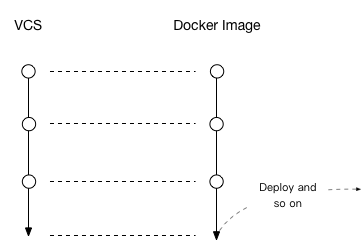
\includegraphics[width=0.7\textwidth]{detail/vcs.png}
  \caption{Fornax版本管理系统管理模块UML类图}
  \label{fig:vcs}
\end{figure}

由图\ref{fig:vcs}所示,版本管理系统管理模块向外暴露两个接口,分别对应着Clone操作和给一个指定的分支打上标签的操作。这两个操作会在异步事件管理模块处理相应事件时被调用。而为了满足适配多种版本管理系统的要求,版本管理系统管理模块将所有对于版本管理系统的操作抽象成了一个接口,由接口定义了一系列标准地,Fornax需要调用版本管理系统来支持的功能。而不同的版本管理系统需要分别实现对应的功能,以满足接口的要求。而对于版本管理系统的封装与版本管理系统管理模块是解耦合的,当需要使用其进行相应操作时,版本管理系统管理模块会根据用户的设定,先创建出操作对应的版本管理系统的对象,然后根据该对象进行操作。目前所有版本管理系统的实现是通过在go语言中调用Shell程序,来使用本地的版本管理系统的命令行工具来进行支持的。所以版本管理系统的封装本身是无状态的,因此重复创建并不会带来太大的开销。

一方面,go语言作为一门新兴的语言,目前没有能满足Fornax需求的对版本管理系统进行操作的第三方库支持,另一方面,调用Shell的方法可以满足现在的需求。所以Fornax采取了这样的方式来解决对于版本管理系统的依赖,在之后的愿景中,Fornax希望借助第三方库的支持,能够对版本管理系统进行更加准确地定义和使用。

\section{持续集成管理模块}

持续集成管理模块是Fornax中较为复杂的模块之一。其职责不仅包括对代码执行持续集成,还有对于除了构建与发布镜像之外的所有在创建版本时需要进行的操作,比如构建前的钩子,构建后的钩子,以及发布管理等等。因此这样的命名不能反应其明确的功能,但是在Fornax中还是以这样的方式去命名的,因为在最初时它只是为了进行持续集成而存在的。

\subsection{配置文件解析}

因为持续集成管理模块贯穿了创建版本流程的始终,因此对于该模块的实现介绍将从创建版本的流程出发。在创建版本的过程中,第一步是将仓库的代码进行Clone,接下来是解析代码中的配置文件。配置文件是用户定义的,与代码存放在相同目录下的一个YAML格式的文件。Fornax定义了一种语法与惯例,使得用户在按照语法将自己的需求以YAML文件的形式描述后Fornax可以根据该文件执行相应的操作。该文件默认名为caicloud.yml,如果在用户的仓库中存在以此命名的文件,Fornax会尝试解析该文件。这是持续集成管理模块的第一项职责。

\begin{lstlisting}[caption={配置文件实例}]
integration:
  services:
    mongo:
      image: mongo:2.4
      command: mongod
  image: golang:1.5
  volumes:
    - .:/go/src/github.com/gaocegege/the-big-brother-is-watching-you
  env:
    - GOPATH=/go
  commands:
    - pwd
    - ls
    - go get github.com/tools/godep
    - godep go build -race .
    - ./the-big-brother-is-watching-you --mongo-db-ip=mongo
\end{lstlisting}

代码所示是一个完整的配置文件。其中包括了五个阶段的配置信息,分别是持续集成、构建前、构建与发布、构建后、以及发布。在Fornax中,整个创建版本的过程都是由该配置文件进行控制的。用户可以通过定义各个阶段的配置,来确定构建阶段的行为。持续集成管理模块会对该配置文件进行解析,将其解析为一个运行时的树状结构,然后逐一执行。解析过程与传统编译器的词法分析器和语法分析器的实现类似,通过将配置文件的结构以结构体的形式定义,将配置文件解析为树状结构。树状结构可以直接被持续集成管理模块中的运行时所解释,从而根据配置执行相应的任务。

\subsection{执行树构建}

\begin{table}[!hpb]
  \centering
  \caption{语法树节点类型}
  \label{tab:nodetype}
  \begin{tabular}{ll} \toprule
    节点类型 & 描述 \\ \midrule
    NodeList & 根节点类型,用以构造多叉树 \\
    NodePreBuild & 构建前节点类型  \\
    NodeBuild & 持续集成中有关构建的节点类型  \\
    NodePostBuild & 构建后节点类型 \\
    NodeService & 持续集成中有关服务的节点类型  \\ \bottomrule
  \end{tabular}
\end{table}

执行树是一个多叉树结构,是由配置文件解析生成的,运行时执行的一个树状结构。表\ref{tab:nodetype}是树状结构中的节点类型。其中根节点是一个以节点为元素的列表。而其他节点类型都是以节点形式存在于该列表中。目前,执行树的深度最大为一,即所有的节点都直接与根节点相连。除了根节点外,其余所有节点都是一个包含了部分用户的配置信息的节点。而配置信息与节点的对应关系并不是一对一的,比如持续集成节点就对应着零个或多个服务节点,以及一个构建节点。因此执行树并不是一个语法树,而是一个由语法树得到的为了运行时而存在的结构。

运行时的环境除了执行树之外,还有一些用来进行资源隔离,以及与数据库等进行交互的对象。这些对象共同构成了持续集成管理模块的运行时环境。在运行时,除了根节点之外,所有的节点都与一个Docker容器对应。不同的阶段都对应着一个或者多个Docker容器,因此持续集成、构建前和构建后的钩子等等功能,都是通过Docker的容器机制实现的。

\begin{figure}[!htp]
  \centering
  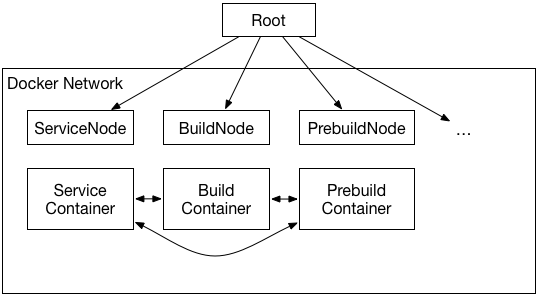
\includegraphics[width=0.7\textwidth]{detail/tree.png}
  \caption{Fornax执行树模型}
  \label{fig:tree}
\end{figure}

使用容器来执行各个阶段的任务,是出于资源隔离的考虑。容器本身具有轻量级,隔离性较好等特性,非常适合用来处理构建任务。构建任务需要在任务内所有的资源共享而构建任务之间应该具有良好地资源隔离性。为了实现这一要求,Fornax在网络,处理器,内存等的使用上都做了一些处理。首先从网络层面,为了保证构建内的所有容器可以相互交互而构建外的容器不可感知到其存在,Fornax使用了Docker的网络特性,为每一次构建都新建了一个Docker的网络。如图\ref{fig:tree}所示,在一次构建内,所有的容器都在一个为构建任务新建的Docker的网络中。在网络中,所有的容器都可以通过容器的名字或者定义的别名去对其他容器进行服务发现,这是由DNS的名字解析来实现的。而在同一个Docker Host中不允许有同名的容器,因此为了解决名字冲突问题,Fornax对需要暴露服务的容器会将其的名字以网络中的别名的形式出现,而对于容器名则进行一定的随机以保证不存在名字冲突。因此对于容器而言,其不感知自己名字而可以通过别名的方式让其他的容器与其进行交互。

引入Docker的网络是为了解决网络的隔离问题,而处理器和内存的隔离问题的解决相对而言要简单很多。容器本身在运行时就支持指定一定的处理器与内存配额,其实现方式取决于容器引擎的实现。目前Docker是依赖内核中的一些特性来实现的,其功能已经可以满足Fornax对隔离性的要求。因此Fornax会在启动容器时指定容器可用的最大处理器与内存配额,在之后Fornax的愿景是可以根据构建任务的需求,允许用户在一定的范围内指定配额,或者向用户推荐其最合适的配额。

除此之外,使用容器技术解决隔离问题,会涉及到代码目录应该如何映射到容器中的问题。因为对于一次构建而言,会有多个容器被启动。因此在容器中进行Clone是低效的选择,而Fornax使用Docker的数据卷特性,先把代码仓库Clone到本地,之后绑定到容器中,这样的实现方式也使得容器对于目录的修改会被保留在本地,在整个创建版本的流程中所有的工件都可以保留下来。

\subsection{持续集成}

持续集成是持续集成管理模块中比较重要,也是实现难度比较大的一个功能,对于持续集成的支持是Fornax在设计之初最重要的需求之一。对于用户代码的持续集成,不仅是允许用户对其代码执行一些简单的测试,也要同时支持在测试同时将用户的环境依赖运行起来,满足一些端到端测试的需要。因此,在持续集成中,也存在一个服务的概念。此处的服务与Fornax中的服务并不是同一概念,Fornax中的服务是与用户的仓库相对应的一个概念,代表了用户的一个功能模块。而在持续集成中的服务,是指用户的代码在运行时的环境依赖。比如一个典型的网站应用,会由前端、后端服务器和数据库组成,而对于前端的端到端的测试,需要将后端的服务器和数据库运行起来才能进行,而在持续集成的概念里,后端的服务器与数据库在此时即可被视为服务。而Fornax支持用户的持续集成对于服务的依赖,是使用容器技术来对其进行支持的。

在之前的配置文件一节中,配置持续集成不仅可以指定持续集成的命令,环境变量等,还有一个其他的阶段都不存在的配置,即服务配置。用户可以通过定义服务配置,在持续集成时先将服务运行起来,随后再执行定义的持续集成命令。因此在持续集成阶段,会有多个容器被启动,容器之间都会被加入到同一个Docker的网络中以相互通信。在持续集成结束后,Fornax会先将所有的容器都删除,之后再将构建中使用的Docker的网络删除,保证没有构建垃圾的残余。如果持续集成完成,会继续执行树结构上的其他节点,完成创建版本的流程,而如持续集成失败,就会返回错误,结束所有流程。因为对于构建垃圾的清理,以及数据库操作等都是以异步事件管理模块中的钩子来实现的,所以无论成功与否,都不会留下残留的垃圾,这也是异步事件管理模块在设计上的一种好处。

在持续集成时,持续集成管理模块会与Docker管理模块共用一个Docker Client对象,因此目前Docker管理模块与持续集成管理模块会有所耦合。

\subsection{构建时钩子}

Fornax支持构建前和构建后的钩子,由于两者所运行的时间不同,因此有不同的实现。对于构建前的钩子而言,往往是为了配合构建。在有关Docker的生产实践中,两个Dockerfile完成构建的应用场景越来越多,而这样的应用场景只通过构建与发布的过程,并不能得到满足。而引入了构建前的钩子,就可以满足这样的需求。在实现上,Fornax会在持续集成结束后,再次根据构建前的钩子运行一个容器,该容器会执行在配置中定义的内容,而且采取了绑定目录的方式解决目录问题,所以在构建前的钩子中所产生的输出在构建时刻都是可见的。

构建后的钩子是为了执行一些用户定义的发布任务。因为在一些应用场景中,用户不仅仅需要产出一个版本镜像,还会有一些自定义的内容需要发布,构建后的钩子就是来解决这样的需求的。相比于其他的步骤而言,其实现较为简单,以一个容器的方式运行,并且执行用户定义的脚本。

\subsection{部署}

除了构建与发布之外,所有的环节都由配置文件所控制。因此在部署时,也是由用户在配置文件中写明要部署的具体集群与位置,Fornax会负责与其后的容器集群进行交互,完成部署任务。在部署时,是通过集群的REST API与其进行交互。因此相对于容器集群而言,Fornax是一个服务的前端,用户可以通过原本的方式进行部署,也可以在Fornax中使用配置的方式完成自动部署。

\section{Docker后台管理模块}

Docker后台管理模块是为了更好地解决并发构建而引入的模块。通过Docker网络的支持,Fornax使得每次构建之间不会出现端口的冲突,而这并不能完全解决并发的构建问题。除此之外,还存在一个问题,就是在同一时间内的同一个镜像,Docker只允许有一个镜像被推送,而这样是不能满足Fornax的需求的,因此需要引入Docker后台管理模块来解决该问题。

Docker后台管理模块是在开发的后期被引入的一个模块,它会管理多个连接不同Docker Host的Docker管理模块,可以被理解为是维护一个可用的Docker管理模块的资源池的模块。当需要使用Docker管理模块进行镜像的构建与发布时,Fornax会向Docker后台管理模块请求一个空闲的Docker管理模块实例,之后的操作中会使用该实例进行镜像的推送与发布。

\section{日志模块}

日志对于Fornax而言的重要性毋庸置疑。而Fornax为了保证日志可以准确而实时地推送给用户前端的同时,保持Fornax的资源高效利用,因此设计了一套基于WebSocket的与客户端进行通信的简易协议。该协议允许Fornax与客户端建立WebSocket连接,在有日志产生时,实时地将日志推送给用户端。同时在用户端一定时间内没有回应时,Fornax会自行关闭该连接,以保证不会因为保持过多的连接造成资源的浪费。

日志模块的实现依赖Kafka,一个使用阿帕奇许可证开源的高吞吐量的分布式消息中间件系统。Kafka支持发布者-订阅者的模式,对一个指定的主题(Topic)进行订阅,订阅者会在有新消息被提交时收到该消息。Fornax会在每次构建时,新建一个Kafka的主题,该主题会对应一次构建,在该构建中的所有日志都会发送至该主题。而Fornax会负责将主题持久化,并且在有订阅者订阅该主题时进行推送。

在Fornax中,通过Kafka实现了对日志的订阅,而与客户端进行交互则是使用了WebSocket连接。WebSocket是在RFC 6455\cite{websocket}中被提出来的一种建立在单个TCP连接上的全双工的通信协议。它允许服务端向用户端主动地推送数据或信息,这正是日志推送所需要的功能。

\begin{figure}[!htp]
  \centering
  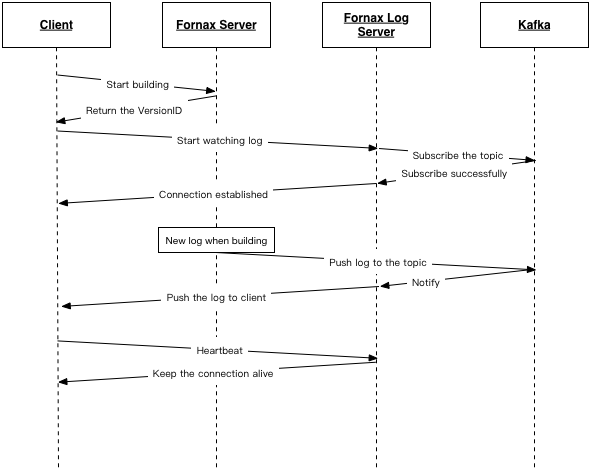
\includegraphics[width=0.9\textwidth]{detail/log.png}
  \caption{Fornax日志模块交互图}
  \label{fig:log}
\end{figure}

为了实现日志实时推送的功能,Fornax在其主线程之外还有一个监听其他端口的日志服务器线程,该服务器只负责有关日志获取的部分逻辑。它从Kafka中获取日志,并将其推送给订阅相关日志的客户端。客户端、Fornax主服务器线程、Fornax日志服务器线程与Kafka之间的交互如图\ref{log}所示,当客户端发起一次构建时,Fornax会先生成一个唯一的标识符代表这次构建产生的版本,而随后会由异步事件管理模块调度构建的运行。在运行时,构建产生的日志会由Fornax推送给Kafka,而指定的主题是由发起构建的用户唯一标识符,构建所在的服务的唯一标识符,和代表该次构建的唯一标识符拼接而成。所有在构建时的日志都会被推送至该主题中。

因此,所有构建时的日志都会推送至Kafka中,而Fornax日志服务器线程,其本质是一个只与Kafka进行交互的独立线程。它会监听一个独立于Fornax主线程的端口,接受来自客户端的请求并处理。当接收到来自客户端的请求时,Fornax日志模块会去订阅相应的日志主题,然后当Fornax在构建时的日志被推送到Kafka中时,日志管理模块就可以订阅到该推送,并借由之前建立的连接推送至客户端,完成日志的推送工作。

为了完成这一步,Fornax设计了一个简单的应用层通信协议,保证日志可以实时准确地推送到客户端的同时不会占用过多的资源。首先,客户端会与Fornax的日志管理模块建立WebSocket连接,以便客户端与Fornax之间进行通信,客户端与Fornax通信的数据格式为JSON。请求与返回的数据包格式如表\ref{tab:protocol-client}和表\ref{tab:protocol-server}所示。在客户端想订阅日志时,会先向Fornax发送一个数据包,该数据包有如表\ref{tab:protocol-client}所示的字段。其中第一个字段动作在客户端发往Fornax的请求中会被置为查看日志,而接口字段会被统一置为创建服务或者创建版本,因为只有在创建服务或者版本时Fornax才有日志被写入Kafka中。而后面的用户、服务、与版本的唯一标识符是为了确定请求对应的具体日志。此时是客户端向Fornax发送的第一个包,用以通知Fornax该客户端希望订阅一个具体的日志。因此请求包中的日志字段为空,操作字段会被置为开始,以通知Fornax该客户端希望开始接收该次构建的日志推送。而唯一标识符则是唯一的标识该包的字段,会被设为一个自动生成的通用唯一识别码(Universally Unique Identifier)。通用唯一识别码的目的在于唯一的标识该包,在客户端与Fornax密集通信时保持请求与回应的一致。

\begin{table}[!hpb]
  \centering
  \caption{Fornax日志模块请求的数据包格式}
  \label{tab:protocol-client}
  \begin{tabular}{ll} \toprule
    字段 & 说明 \\ \midrule
    action & 动作 \\
    api & 接口 \\
    user\_id & 用户名 \\
    service\_id & 服务唯一标识符 \\
    version\_id & 版本唯一标识符 \\
    log & 日志内容 \\
    operation & 操作 \\
    id & 唯一标识符 \\ \bottomrule
  \end{tabular}
\end{table}

\begin{table}[!hpb]
  \centering
  \caption{Fornax日志模块返回的数据包格式}
  \label{tab:protocol-server}
  \begin{tabular}{ll} \toprule
    字段 & 说明 \\ \midrule
    action & 动作 \\
    reponse & 返回 \\
    id\_ack & 请求的唯一标识符 \\
    error\_code & 错误码 \\
    error\_msg & 错误信息 \\ \bottomrule
  \end{tabular}
\end{table}

在Fornax收到动作字段为查看日志的请求包,并且该包中操作字段为开始时,会返回一个包以表示收到该请求包,返回的包格式如表\ref{tab:protocol-server}所示,在返回的包中,动作字段统一会被置为返回,而返回字段会被置为收到请求,请求的唯一标识符字段会被置为之前请求包中自动生成的通用唯一识别码,而错误码为零,错误信息会置为成功。与此同时,日志模块会创建一个新的线程,并且在线程中创建一个Kafka的消费者对象,该对象会订阅根据请求中用户、服务、版本三个唯一标识符而确定的唯一的日志主题,随后会向与客户端建立的会话中推送包含日志信息的数据包。这是由Fornax主动推送给客户端的包,其格式与客户端向Fornax发起的请求包格式一致,但字段的值会有所不同。其动作字段会被置为推送日志,而不是查看日志。而接口字段仍然与客户端的请求包中保持一致,其后的用户、服务、版本三个唯一标识符也同样与客户端的请求包中保持一致。而相比于客户端向Fornax发送的请求包,两者最大的不同在于其日志字段不再为空,而是会根据Kafka中订阅的主题获得的日志数据来进行发送。客户端在接收到Fornax发送的日志推送包时,会返回一个格式如表\ref{tab:protocol-server}所示的包,以通知Fornax该包已经被接收。

在Fornax中,日志模块是运行在一个单独的线程中的。在日志写入Kafka的部分实现中,是使用了本地与Kafka相互配合的方式来进行的。首先,关于构建的日志会写入到一个临时文件中,这是最开始Fornax的实现。而在开发中发现将日志信息存储在本地不利于Fornax的分布式部署,因此在之后的实现中引入了Kafka的依赖。在引入Kafka后,Fornax同样会先将日志信息存储在本地的文件中,而在每次构建时,会启动一个新的线程去监听日志文件的变化。目前监听的实现方式是轮询,每隔一定的时间间隔Fornax会重新访问本地的临时日志文件,将变动以消息的方式发送给Kafka。日志写入Kafka的实现是日志模块与Fornax主要功能想耦合的一部分,在进行构建时会调用该部分实现进行日志的写入。

而将日志发送给客户端是独立于Fornax主要功能的实现,是一个单独的服务器线程。在该部分实现中,日志模块会启动一个监听端口的服务器,并维护一个活跃的WebSocket连接的会话列表。该服务器只提供一个接口,即建立客户端与日志模块的连接。在连接建立后,日志模块会直接通过连接与客户端进行交互。日志模块在交互时定义了两个通信的接口,分别是查看日志与发送心跳。客户端可以对日志模块发送这两种类型的请求包,其中查看日志是前文中提到的由客户端第一次发给Fornax日志模块的请求包,而心跳是为了维持连接而由客户端定时地发送给Fornax日志模块的请求包,心跳请求会更新对应会话的最后活跃时间。

从实现来看,日志模块是一个相对独立于Fornax的模块,在后续对分布式部署实现的分析时会说明这样设计的目的。

\section{数据库管理模块}

数据库管理模块,是Fornax与MongoDB进行交互的操作对象。在实现上,一共由两个管理器构成,即服务管理器与版本管理器。在Fornax被启动时,在初始化时会创建两个管理器的全局实例,随后会在API模块以及异步事件管理模块等模块中被使用。该模块的实现较为简单,是一层对于MongoDB中Collection的操作的封装。使得Fornax可以在代码中直接操作MongoDB中的对象。

% 如图\ref{}所示,在Fornax的数据库设计中,一共有两个Collection,分别是服务与版本。